\documentclass[12pt]{article}
\usepackage{inputenc}
\usepackage{graphicx}
\usepackage{tabularx}
\usepackage{hyperref}

%%%%%%%%%%%%%%%%
% Impostazioni %
%%%%%%%%%%%%%%%%

\hypersetup{
    colorlinks=true,
    linkcolor=blue,
    filecolor=magenta,
    urlcolor=cyan,
    pdftitle={Database Autoveicoli, Michael Guidelli},
    pdfpagemode=FullScreen,
}

\date{}

\begin{document}

%%%%%%%%%%
% Titolo %
%%%%%%%%%%

\maketitle
\null \null \null \null \null \null
{\centering
    \huge\bfseries Database Autoveicoli \\
    \Large\normalfont Michael Guidelli  \\
}

\clearpage

%%%%%%%%%%%%%%%%%%%%%
% Traccia esercizio %
%%%%%%%%%%%%%%%%%%%%%

\section*{Traccia esercizio}

\noindent
Si desidera realizzare il database degli autoveicoli e dei loro proprietari di un certo paese, ricordando che
un autoveicolo può essere anche di proprietà di più persone (co-intestazione). In particolare si vuole
registrare anche quale tipo di alimentazione abbia ogni veicolo; le possibilità di alimentazione devono
essere le seguenti: benzina, diesel, gpl, metano, elettrico, idrogeno, ibrido (per considerare autoveicoli
alimentabili con più tipi di propellenti). Aggiungere le eventuali ipotesi necessarie. E' richiesto di
realizzare lo schema ER e lo schema logico.

\clearpage

%%%%%%%%%%%%%%%%%%%%%%%%%%%%%%%%
% Impostazioni indice e figure %
%%%%%%%%%%%%%%%%%%%%%%%%%%%%%%%%

\renewcommand{\contentsname}{Indice \label{indice}}
\tableofcontents

\renewcommand{\listfigurename}{Lista delle figure}
\listoffigures

\renewcommand{\listtablename}{Liste Attributi}
\listoftables

\clearpage

%%%%%%%%%%%%
% Premesse %
%%%%%%%%%%%%

\section{Premessa}

\noindent
Ipotizzando di star realizzando un database per la motorizzazione della regione/paese di residenza, posso ipotizzare che il database abbia bisogno delle seguenti informazioni: \newline

\subsection{Informazioni riguardanti le automobili:}
\begin{enumerate}
    \item colore;
    \item targa;
    \item anno di produzione;
    \item alimentazione; 
    \item modello;
    \item numero telaio \textbf{(attributo identificativo)};
\end{enumerate}

\subsection{Informazioni riguardanti i proprietari:}
\begin{enumerate}
    \item nome;
    \item cognome;
    \item età;
    \item nazionalità;
    \item codice fiscale \textbf{(attributo identificativo)};
\end{enumerate}

\noindent
Si ipotizza che la motorizzazione abbia bisogno delle sudette informazioni per registrare autoveicolo e proprietario.

\clearpage

%%%%%%%%%%%
% Ipotesi %
%%%%%%%%%%%

\section{Ipotesi}
\begin{enumerate}
    \item Se l'autoveicolo è dotato di motore ibrido l'attributo dello stesso sarà appunto di tipo ibrido non tenendo conto della tipologia.
\end{enumerate}

%%%%%%%%%%%%%%%%%%%%%%%%%%%%%%%%%%%%%%%%%%%%
% Criterio scelta attributo identificativo %
%%%%%%%%%%%%%%%%%%%%%%%%%%%%%%%%%%%%%%%%%%%%

\section{Criterio scelta attributo identificativo}
\noindent
Ho scelto nel caso dell'autoveicolo il numero del telaio perché è univoco e non nullo (In alternativa si può utilizzare la targa). \newline
Ho scelto nel caso dei proprietari il codice fiscale perché è univoco e non nullo.

\clearpage

%%%%%%%%%%%%%%
% Modello ER %
%%%%%%%%%%%%%%

\section{Modello ER}

\begin{center}
    \begin{figure}[h!]
    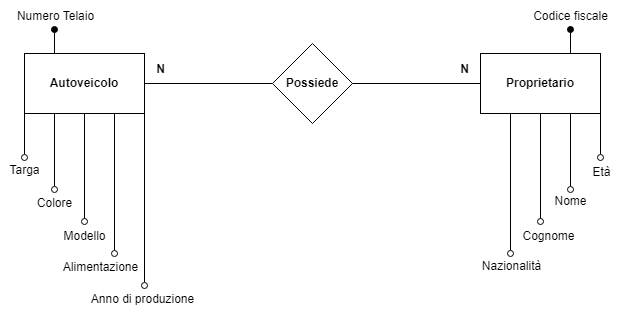
\includegraphics[width=14cm]{modello_er_autoveicolo.png}
    \caption{Rappresentazione modello ER}
    \label{fig: Modello ER}
\end{figure}
\end{center}


\subsection{Cardinalità}
\noindent
Cardinalità delle associazioni:

\begin{itemize}
    \item \textbf{Possiede}: in questo la caso la cardinalità è \textbf{N} a \textbf{N} perché ciascun singolo autoveicolo può essere posseduto da uno o più proprietari e ciascun singolo proprietario può possedere più autoveicoli.
\end{itemize}

\clearpage 

%%%%%%%%%%%%%%%%%%%%%%%%%%%
% Tabella degli attributi %
%%%%%%%%%%%%%%%%%%%%%%%%%%%

\begin{center}
    \section{Liste degli attributi}
\end{center}

% entità autoveicolo % 

\subsection*{Entità Autoveicolo}
\begin{table}[h!]
    \centering
    \begin{tabular}{|c|c|c|c|}
        \hline
        Nome attributo & Significato & Tipo di dato & Vincolo \\
        \hline
        Numero Telaio & Attributo identificativo & Varchar & Max 17 caratteri \\
        \hline
        Targa & Targa dell'auto & Varchar & Max 7 caratteri \\
        \hline\
        Colore & colore auto & Varchar & Max 255 caratteri \\
        \hline
        Anno di produzione & Anno produzione auto & Int & Max 4 cifre \\
        \hline 
        Alimentazione & Tipo alimentazione auto & Varchar & Max 255 caratteri \\
        \hline
        Modello & Modello auto & Varchar & Max 255 caratteri \\
        \hline
    \end{tabular}
    \caption{Lista Autoveicolo}
    \label{tab:my_label}
\end{table}

% entità proprietario %

\subsection*{Entità Proprietario}
\begin{table}[h!]
    \begin{tabular}{|c|c|c|c|}
        \hline
        Nome attributo & Significato & Tipo di dato & Vincolo \\
        \hline
        Codice fiscale & Attributo identificativo & Varchar & Max 16 caratteri \\
        \hline
        Cognome & Cognome proprietario & Varchar & Max 255 caratteri \\
        \hline
        Nome & Nome proprietario & Varchar & Max 255 caratteri \\
        \hline
        Età & Età proprietario & Varchar & Max 255 caratteri \\
        \hline
        Nazionalità & Nazionalità proprietario & Varchar & Max 255 caratteri \\
        \hline
    \end{tabular}
    \caption{Lista Proprietario}
    \label{tab:my_label}
\end{table}

\end{document}